\chapter{Deformed Nuclei}

\section{Nuclear deformation}

Most of the nuclei across the nuclide chart are spherical or symmetric in their ground state. Moreover, for the axially symmetric nuclei (i.e, either \emph{oblate} or \emph{prolate}), there is a prolate over oblate dominance. In Figure \ref{nuclear_shapes}, the nuclear shapes are shown.

\begin{figure}[ht]
    \centering
    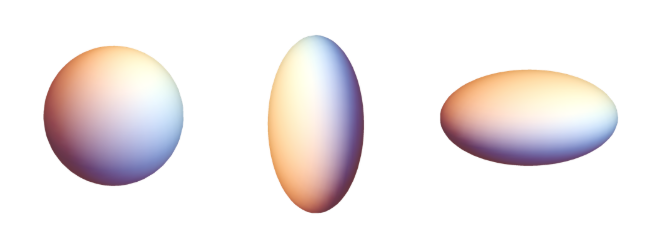
\includegraphics[scale=0.3]{Chapters/Figures/nuclear_shapes.png}
    \caption{Nuclear Shapes.}
    \label{nuclear_shapes}
\end{figure}

The spherical shell model only describes nuclei near the closed shells. On the other side, for the nuclei that lie far from closed shells, a deformed potential must be employed. 
In the case of even-even nuclei, unique band structures resulting from the vibrations and rotations of the nuclear surface (as proposed by Bohr and Mottelson \cite{bohr1998nuclear} in the \emph{Geometric Collective Model} - GCM) appear in the energy range 0-2 MeV.

Within the GCM, the nucleus is described as a classical charged liquid drop.